\documentclass[12pt]{article}
\usepackage{caption}
\usepackage{caption}
\usepackage[utf8]{inputenc}
\usepackage[german]{babel}
\usepackage{graphicx}
\usepackage{svg}	
\usepackage{listings}
\usepackage{url}
\usepackage{xcolor}
\usepackage{textcomp}
\usepackage{fancyhdr}
\usepackage{comment}
\usepackage[onehalfspacing]{setspace}
\bibliographystyle{ieeetr}
\usepackage[left=4cm,right=2cm,top=4cm,bottom=2cm,includeheadfoot]{geometry}

\graphicspath{{images/}}

\captionsetup[table]{position=bottom}

\lstset { %
    language=C++,
    backgroundcolor=\color{black!5}, % set backgroundcolor
    basicstyle=\footnotesize,% basic font setting
}


\DeclareCaptionType{code}[Code Listing][List of Code Listings] 


\pagestyle{fancy}
\fancyhf{}
\fancyhead[L]{\rightmark}
\fancyhead[R]{\thepage}
\renewcommand{\headrulewidth}{1pt}

\begin{document}
\begin{titlepage}
	\centering
	
\includegraphics[width=0.3\textwidth]{logo}\par\vspace{1cm}
	{\scshape\LARGE Hochschule für Angewandte Wissenschaften Hof \par}
	\vspace{1cm}
	{\scshape\Large Seminararbeit\par}
	\vspace{1.5cm}
	{\huge\bfseries Aufbau und Funktionsweise eines Prozessors\par}
	\vspace{2cm}
	{\Large\itshape Marco Vogel\par}
	\vfill
	unter Aufsicht von\par
	Stefan Müller
	\vfill
% Bottom of the page
	{\large\today\par}
\end{titlepage}
\newpage


\tableofcontents
\newpage
\listofcodes




\section{Motivation}
\section{Zahlensysteme}
Unser geläufiges Zahlensystem ist das Dezimalsystem. Das bedeuted, dass Zahlen mit folgender Formel gebildet werden:
$$Z=\sum\limits_{i=0}^{n-1} a_i * 10^i$$
Somit wird die Dezimalzahl 135 folgendermaßen gebildet:$$Z=1*10^2+3*10^1+5*10^0 = 135$$
Die Basis der Wertepotenz spiegelt das Zahlensystem wieder welches dargestellt wird, weshalb die Formel im Allgemeinen darstellbar ist für die Zahl $Z$ mit Basis $B$:
$$Z=\sum\limits_{i=0}^{n-1} a_i * B^i$$
Das dezimale Zahlensystem ist für Menschen sehr intuitiv zu verstehen. Da wir zehn Finger haben können wir optimal mit diesem Dezimalsystem zählen. Für Computer ist dieses Zahlensystem allerdings ungeeingnet. Ein Prozessor besteht aus vielen kleinen Transistoren, diese können entweder Strom fliesen lassen oder nicht. Somit bietet sich ein Zahlensystem an, welches nur zwei Zustände kennt. AN und AUS, Strom kann fliesen oder Strom kann nicht fliesen. Der deutsche Mathematiker Gottfried Wilhelm Leibniz entwickelte die Dyadik, die Darstellung von Zahlen durch 1 und 0. Diese Darstellungsform ist für Prozessoren viel intuitiver, da sie selbst ebenfalls nur zwei Zustände kennen.\cite{wiki:dual}.
%HEX-System vllt noch
\subsection{Binäre Darstellung von Zahlen}
Zahlen im Dualsystem können vorzeichenlos und vorzeichenbehaftet dargestellt werden.Vorzeichenlose Binärzahlen können mittels folgender Formel gebildet werden: $$Z=\sum\limits_{i=0}^{N-1} a_i * 2^i$$ 
Die Dezimalzahl 135 würde dann im Dualsystem dem Bitmuster $10000111$ entsprechen, dargestellt durch folgende Konvertierung:
$$10000111b = 1*2^7+0*2^6+0*2^5+0*2^4+0*2^3+1*2^2+1*2^1+1*2^0 = 128 +4+2+1 = 135d$$
Prozessoren haben immer eine begrenzte Anzahl an Bits zur Verfügung mit denen sie arbeiten können. Deshalb kann es während der Ausführung mit vorzeichenlosen Zahlen zu einem Überlauf kommen. Ein Überlauf tritt auf, wenn zum Beispiel auf einer 8-Bit CPU die Operation 255+1 ausgeführt wird, da als Ergebnis 0 geliefert wird. 
Das geschieht, da die Zahl 255s die Dualdarstellung $11111111$ besitzt. Da 255d die größte darstellbare Zahl in 8-Bit ist wird die Addition von 1 einen Fehler verursachen. Das Ergebnis $256d$ benötigt zur dualen Darstellung 9 Bit($100000000b$), allerdings können nur 8 Bit gespeichert werden. Deshalb werden die ersten 8 Bit verwendet und das Ergebnis ist 0.


\begin{table}[!htb]
\centering
\caption{Rechnung mit Übertrag}
\label{my-label}
\begin{tabular}{|c|r|r|}
\hline
\textbf{Übertrag}               & \multicolumn{1}{c|}{\textbf{Binär}} & \multicolumn{1}{c|}{\textbf{Dezimal}} \\ \hline
-                               & 11111111b                            & 255d                                   \\ \hline
-                               & 00000001b                            & +1d                                     \\ \hline
\multicolumn{1}{|r|}{1}         & 00000000b                            & 256d                                   \\ \hline\hline
\multicolumn{1}{|r|}{Ergebnis:} & 00000000b                            & 0d                                     \\ \hline
\end{tabular}
\end{table}
Diese Rechenoperation würde in der CPU das Carry Flag (Übertragsbit) setzen um dem Programmierer darauf hinzuweißen, dass die letzte Operation keine richtigen Werte erzeugt hat. Den vorzeichenlosen Dualzahlen fehlt allerdings die Möglichkeit, negative Werte anzunehmen. Diese Eigenschaft bieten vorzeichenbehaftete Dualzahlen. Eine Dualzahl im sogenannten Zweierkomplement wird folgendermaßen gebildet:
$$Z=-a_{N-1}*2^{N-1}+\sum\limits_{i=0}^{N-2} a_i * 2^i$$
Die Formel kann zu Erklärungszwecken in zwei Teile gegliedert werden. Zum einen die erste Teil $-a_{N-1}*2^{N-1}$, das Vorzeichenbit. Dieser sagt aus, dass das höchstwertige Bit einer vorzeichenbehafteten Zahl negativ gewertet wird. Der hintere Teil $\sum\limits_{i=0}^{N-2} a_i * 2^i$ ist bereits aus der Erzeugung von vorzeichenlosen Dualzahlen bekannt. Die Bits werden nach ihrer Position gewichtet und ihre Wertigkeit aufaddiert. Die Zahl $10000111b$ im Zweierkomplement wird also wie folgt interpretiert:
$$10000111b = -1*2^7+0*2^6+0*2^5+0*2^4+0*2^3+1*2^2+1*2^1+1*2^0 = -128+4+2+1 = -121d$$
Bei den vorzeichenlosen Dualzahlen konnte es, wie oben beschrieben, zu einem Übertrag kommen, wenn der darstellbare Zahlenbereich überschritten wurde. Ein ähnliches Verhalten besitzen Zahlen im Zweierkomplement, allerdings kommt es zu einem Überlauf statt einem Übertrag. Zur Erklärung soll der 8-Bit Prozessor die Rechnung 127+1 durchführen. Hier wird nun nicht 128 als Ergebnis geliefert, sondern -128. Dies geschieht aufgrund der Interpretation von vorzeichenbehafteten Dualzahlen. Da das vorderste Bit nun gesetzt ist, interpretiert der Prozessor die Wertigkeit nun mit -128 statt 128, und da die restlichen sieben Bit null sind wird das Ergebnis als -128 interpretiert.

\begin{table}[!htb]
\centering
\caption{Rechnung mit Überlauf}
\label{my-label}
\begin{tabular}{|c|r|r|}
\hline
\textbf{Überlauf}               & \multicolumn{1}{c|}{\textbf{Binär}} & \multicolumn{1}{c|}{\textbf{Dezimal}} \\ \hline
-                               & 01111111                            & 127                                   \\ \hline
-                               & 00000001                            & +1                                    \\ \hline
Ja                              & 10000000                            & -128                                  \\ \hline\hline
\multicolumn{1}{|l|}{Ergebnis:} & 10000000                            & -128                                  \\ \hline
\end{tabular}
\end{table}



\section{Logische Schaltglieder}
\subsection{AND-Gatter}
\subsection{OR-Gatter}
\subsection{NOR-Gatter}
\subsection{XOR-Gatter}
\subsection{NOT-Gatter}
\subsection{Flip-Flops}

\section{Prozessorarchitekturen}
Mikroprozessoren besitzen immer einen eigenen, meist einzigartigen, Aufbau. Allerdings haben sich im Laufe der Entwicklung einige Architekturmerkmale ausgeprägt, welche die Prozessoren verbindet. 
Ziel dieser Architekturen ist es stets, die Ausführungsgeschwindigkeit eines Programmes zu beschleunigen.
\subsection{Von-Neumann Architektur}
Die Von-Neumann Architektur ist nach dem ungarisch-US-amerikanischen Mathematiker John von Neumann benannt. Er hat 1945 in dem Bericht (First Draft of a Report on the EDVAC) das Prinzip erstmals beschrieben.
Die Von-Neumann Architektur besteht grundlegend aus folgenden Komponenten(siehe Abbildung \ref{fig:vonNeumann}):
\begin{itemize}
\item CPU 
\item Speicherwerk 
\item Ein-/Ausgabewerk
\item Bus-System
\end{itemize}

\begin{figure}[!htb]
\centering
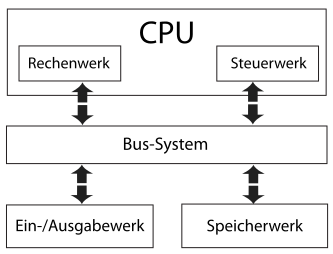
\includegraphics[scale=0.60]{Von-Neumann_Architektur}
\caption{Komponenten Von-Neumann Architektur}
\centering
%TODO vhttps://de.wikipedia.org/wiki/Von-Neumann-Architektur#/media/File:Von-Neumann_Architektur.svg
\label{fig:vonNeumann}
\end{figure}
Bevor John von Neumann dieses Architekturprinzip beschrieben hatte musste für eine bestimmte Aufgabe ein speziell darauf ausgelegter Rechner entworfen und gebaut werden. Mit der Von-Neumann Architektur war das nicht mehr nötig, es konnten verschiedene Programme auf dem gleichen Prozessor ausgeführt werden. Diese Funktion gab dem Prinzip den Namen programmgesteuerter Universalrechner( Stored-Program Machine )\cite{TaschenbuchMikroprozessortechnik}.
Ein sehr zentrales Prinzip dieser Archtitektur ist die Speicherung von Programmcode und Daten im gleichen Speicher. Das führt allerdings auch zu dem Problem, dass die CPU nicht unterscheiden kann ob geladenene Bytes Programmcode oder Daten enthalten. Diese Unterscheidung muss also der Programmierer vornehmen. Außerdem kann mit dieser Archtitektur nur jeweils Daten oder Code geladen werden und somit nur ein Befehl ausgeführt werden. Dieser Umstand erfordert einen speziellen Programmablauf der CPU, den so genannten Von-Neumann Zyklus. Dieser besteht aus den folgenden fünf Schritten welche nacheinander abgelaufen werden.
\begin{enumerate}
\item Instruction Fetch 
\item Instruction Decode
\item Fetch Operands
\item Execute
\item Increment Program Counter (PC)
\end{enumerate}
Im ersten Schritt wird aus dem Speicher der zu abzuarbeitende Befehl in das Befehlsregister geladen. Daraufhin wird im zweiten Schritt der Befehl vom Befehlsdekodierer verarbeitet und die nötigen Steuersignale an die CPU Komponenten weitergeleitet. Dann werden die Operanden welche für den Befehl benötigt werden geladen. Im vierten Schritt wird der Befehl schließlich von der ALU ausgeführt. Im letzten Schritt wird der Befehlszähler (Program Counter - PC) inkrementiert damit er im nächsten Zyklus bereits die Adresse des nächsten auszuführenden Befehls enthält.

\cite{unikoelnvnz}.
%TODO http://hki.uni-koeln.de/archive/hki2016/wisem-2011/basisinformationstechnologie-i/rechnertechnologie-i/arbeitsweise-einer-cpu-von-neumannzyklus.html
\subsection{Harvard Architektur} 
Die Harvard Architektur ist eine abgewandelte Form der Von-Neumann Architektur. Der größte Unterschied besteht darin, Codesegment und Datensegment in separaten Speichern zu verwalten. Diese Konzeption bringt den Vorteil, dass im Gegensatz zur Von-Neumann Architektur Befehle und Daten gleichzeitig geladen werden können. Um diesen Vorteil ausnutzen zu können benötigt ein Harvard Rechner allerdings auch getrennte Daten und Adressbusse. 
\newline
\newline
In modernen x86 Prozessoren ist eine klare Unterscheidung zwischen Von-Neumann und Harvard Architektur nur schwer möglich. So zeigen die modernen CPU sich dem Entwickler zwar als pure Von-Neumann Maschinen, also mit gemeinsamen Code und Datenspeicher (RAM), allerdings besitzen sie intern einen getrennten Level-1 Cache für Instruktionen und Daten, was der Harvard-Architektur entspricht. Die beiden Architekturen haben also jeweils Vor- und Nachteile, wobei in modernen Prozessoren die beiden Konzepte verwendet werden um maximale Leistung zu erzielen.
\subsection{CISC-Prozessoren}
%TODO Geschichte?
Neben den beiden vorherigen CPU-Architekturen gibt es noch zwei weitere Designphilosophien für die Entwicklung von Prozessoren welche sich geschichtlich ergeben haben. In den Anfängen der Prozessorentwicklung gab es einige Faktoren, welche berücksichtigt werden mussten. So wurden Prozessoren bis in die 1970'er Jahre oft in Assembler programmiert. Um den Entwicklern für jeden möglichen Anwendungsfall einen einzelnen Assemblerbefehl zur Verfügung stellen zu können, begannen Prozessorhersteller, immer komplexere Befehle in den Befehlssatz zu integrieren. Diese Befehle beinhalteten oft mehrere Unterschritte, zum Beispiel das Lesen aus dem Speicher und dem Verrechnen zweier Variablen. Um solche Befehle ausführen zu können mussten die komplexen Befehle in mehrere Zwischenschritte aufgeteilt werden, welche dann vom Prozessor nacheinander abgearbeitet wurden. Prozessorhersteller entwickelten deshalb Microcode für den komplexen Befehlssatz, welche einen CISC-Befehl in mehrere Microcode Befehle dekodiert und diese ausführt. Das kostet zwar mehr Platz auf dem Chip für den Befehlsdekodierer, allerdings musste somit nicht mehr oft auf den Befehlsspeicher zugegriffen werden, was sehr viel Zeit kostet. Durch diesen Prozess wuchs die Befehlssatzgröße stark an und wurde immer komplexer. Solch eine ISA (Instruction Set Architecture) wird CISC(Complex Instruction Set Computer) genannt.	
%TODO Struktur überarbeiten.
%TODO http://wiki.osdev.org/Historical_Notes_on_CISC_and_RISC
%TODO https://de.slideshare.net/SuvenduDash/cisc-risc-architecture
\subsection{RISC-Prozessoren}
%TODO Quelle Studie suchen 
Mehrere Faktoren führten dazu, dass die CISC-ISA einige Nachteile entwickelte, weshalb die RISC-ISA (Reduced Instruction Set Computer) entwickelt wurde.


Eine von IBM durchgeführte Studie hat Anfang der 1980er Jahre ergeben, dass Programme, welche auf einer CPU mit CISC ISA liefen, nur einen geringen Teil der zur Verfügung stehenden Instruktionen überhaupt verwenden. Das bedeutet, dass Programme den komplexen Befehlssatz, welche eine CISC CPU bietet, gar nicht ausnutzen sondern nur die simplen und universellen Befehle verwenden. 

Ein weiterer Grund für die Entwicklung der RISC Computer war, dass die Zahl der Entwickler, welche in Assembler programmierten, immer weniger wurden. Mit dem Auftreten der ersten Hochsprachen, insbesondere C, und ihren Compilern, mussten Programmierer nicht mehr den Befehlssatz eines Prozessors kennen. Durch diese Abstraktionsschicht zwischen Prozessor und Programmierer ist die kompakte Struktur von Assemblerbefehlen kein Designfaktor für Prozessoren mehr, da es den Programmierer in den meisten Fällen nicht mehr interessieren musste, wie der erzeugte Assemblercode aussieht.

Des weiteren ist die Latenz zwischen Prozessor und Hauptspeicher in den 1980er Jahren stetig gesunken. Es wurden also deutlich weniger Taktzyklen des Prozessors geopfert, wenn er aus dem Hauptspeicher Befehle anforderte. Dadurch entfiel der Vorteil von nur wenigen Zugriffen auf den Hauptspeicher.

%TODO Quelle unten: Taschenbuch Mikroprozessoren. Seite 85 RISC Ziele
\noindent
Daraus hat sich dann die RISC Philosophie ergeben. Im Gegensatz zu den vorher genannten Punkten implementiert RISC folgende Eigenschaften.

Der Befehlssatz ist auf die wesentlichen Befehle beschränkt. Während CISC Befehlssätze oft 200 oder mehr Befehle beinhalten sind in RISC Befehlssätzen oft nur 100 oder weniger Befehle vorhanden.

Des weiteren wird auf die Mikroprogrammierung verzichtet. Es werden also nicht mehr die Befehle aus dem Befehlsspeicher intern in Mikrobefehle dekodiert. Das spart auf dem Chip Fläche, da der Dekodierer keine komplexen Aufgaben mehr hat. Alle Befehle sind also fest in dem Prozessor implementiert.

Außerdem soll ein Befehl genau einen Takt zur Ausführung benötigen. Wenn bei CISC ein Befehl in mehrere Mikrobefehle dekodiert wird, benötigen diese mehrere Takte bis alle ausgeführt wurden. Dies wird bei RISC vermieden. Jeder geladene Befehl wird dekodiert und spricht genau eine Hardwareeinheit an.

%TODO Quelle: Wüst Seite 102 RISC
Eine weitere Eigenschaft der RISC Philosophie ist die Kommunikation mit dem Hauptspeicher nur über Load und Store Befehle. Dadurch wird die Anzahl der Zugriffe auf den Hauptspeicher reduziert, was die Ausführungszeit senkt. Daraus folgt, dass ein ALU Befehl nur auf Register anwendbar ist, da Register auf Prozessortakt betrieben werden und somit keine Latenz zwischen den beiden Hardwareeinheiten entsteht. Der Befehl, zwei Register zu verrechnen, kann in einem Taktzyklus abgearbeitet werden. Dadurch entfällt wiederum die Notwendigkeit der Mikroprogrammierung. In einer CISC CPU ist zwar eine Speicherverrechnung zwischen Register und Speicherzelle etc. möglich, allerdings nicht skalar, also in einem Takt, sondern in mehreren Teilschritten, zum Beispiel Speicherzelle laden, verrechnen, zurückschreiben.
%TODO Dieser Satz :D Evtl. überarbeiten 
%TODO Auch Wüst Seite 102


Da der Speicherzugriff auch in modernen Prozessoren eine zeitkritische Angelegenheit ist besitzen RISC Prozessoren einen sehr großen Registersatz, üblicherweise 16 oder mehr Register. Das ermöglicht einem Programm, viele seiner Variablen in den Registern zu halten um Hauptspeicherzugriffe zu vermeiden. Hier sind allerdings die Compiler der Programmiersprachen in der Pflicht, optimierten Binärcode für RISC Prozessoren zu generieren. Alle beschriebenen Vorteile erübrigen sich, wenn sie von den Compilern nicht unterstützt werden. Wenn ein für CISC Prozessoren geschriebenes Programm auf einem RISC Prozessor ausgeführt wird, funktioniert es, aber die Variablen werden zum größten Teil im Stack gespeichert, einem Teil des Hauptspeichers, und der Großteil zur Verfügung stehender Register wird nicht verwendet. 
\par
%TODO RISC V verlinken.
Aktuelle Prozessoren sind meist CISC Prozessoren. Mit RISC-V existiert aber ein Projekt welches die Absicht hat wieder moderne und konkurrenzfähige RISC Prozessorendesigns zu entwickeln und als freie ISA zur Verfügung zu stellen . 
\subsection{Klassifizierung}
\subsubsection{Klassifizierung nach Flynn}
\subsubsection{Erlanger Klassifizierung}


\section{Aufbau und Funktion}
\subsection{Register}
Register sind die schnellste Speichereinheit innerhalb einer CPU. Prozessoren besitzen eine vielfach höhere Ausführungsgeschwindigkeit als Arbeitsspeicher. Die CPU müsste ohne Register viele Taktzyklen auf Daten warten bevor sie diese verarbeiten könnte. Register bieten deshalb die Möglichkeit, sehr kleine Datenmengen mit einer sehr geringen Latenz prozessorintern lesen und schreiben zu können. Übliche Registergrößen sind 8,16,32 oder 64 Bit.\cite{mikroprozessortechnik2011} Sie werden aus Flip-Flops aufgebaut welche jeweils genau ein Bit speichern können, das heißt ein 64 Bit Register besteht aus 64 gemeinsam gesteuerten Flip-Flops.\cite{mikroprozessortechnik2011} Diese Art der Datenspeicherung hat allerdings auch einige Nachteile. So verbrauchen Register sehr viel Energie und Platz auf dem Prozessordie, es werden deshalb keine großen Speichermengen zur Verfügung gestellt. (Nachteile evtl streichen)

\subsubsection{Universalregister}
Es werden zwei Arten von Registergruppen unterschieden.In einem Universalregister kann ein Programm Werte und Variablen abspeichern.Sie stehen außerdem einem Programmierer von außen offen, das heißt er kann auf jedes Universalregister direkt zugreifen und seinen Wert verändern.

\subsubsection{Spezialregister}
Spezialregister werden von einer CPU für interne Zwecke genutzt. Oft sind in Prozessoren ähnliche Spezialregister zu finden. 

Der StackPointer(SP) ist ein Register welcher auf die aktuelle Position des Stacks im Speicher zeigt. Wenn der Befehl zu Speicherung eines Werts auf dem Stack ausgeführt wird inkrementiert die CPU automatisch, durch die interne Verschaltung des SP, den Wert des StackPointers. Dadurch zeigt das Register immer auf die nächste freie Speicheradresse im Stack.

Der InstructionPointer(IP) enthält die Adresse des nächsten Befehls im Programmspeicher der ausgeführt werden muss. Auch er wird nach der Abarbeitung eines Befehlszyklus als letzter Schritt inkrementiert. Dieses Register bietet allerdings die Möglichkeit einen anderen Wert zu laden. Das wird zur Realisierung von Sprüngen innerhalb des Programmcodes benötigt. 

Das Statusregister(SR) werden zur Ausführung von bedingten Sprunganweisungen gebraucht. Sie werden auch Flagregister genannt da die ALU, in Abhängigkeit der zuletzt ausgeführten Rechenoperation, einzelne Bit(Flags) setzen kann. Auf die einzelnen Flags und ihre Bedeutung wird im Abschnitt der ALU näher eingegangen
\subsection{Steuerwerk}
Das Steuerwerk ist für die Steuerung von internen Bussystemen des Prozessors zuständig. Es besteht aus zwei wesentlichten Komponenten. Im Befehlsregister (Programm Counter bzw. PC) ist die Adresse des nächsten Befehls enthalten, welcher ausgeführt werden soll. Der Befehl wird von der Adresse des Befehlsregisters in den Befehlsdekodierer geladen und analysiert. Falls nötig wird der Befehl in mehrere Schritte unterteilt, die nacheinander abgearbeitet werden müssen. Ob und wie viele solcher Schritte benötigt werden um einen bestimmten Befehl auszuführen bestimmt zum einen die Architektur des Prozessors und zum anderen der Befehl an sich. Bei RISC Prozessoren 
(\textrightarrow 4.4) ist keine weitere Unterteilung in mehrere Befehle notwendig, bei CISC Prozessoren (\textrightarrow 4.3) besitzt der Befehlssatz sehr viel kompliziertere Befehle welche nicht in einem Takt abgearbeitet werden können. Hier wird der Befehlsdekodierer den Befehl in die nötigen Teilbefehle umwandeln und nacheinander ausführen.




Da über ein Bussystem immer nur zwei Komponenten miteinander kommunizieren können, muss das Steuerwerk die Busse für die jeweiligen Komponenten wie zum Beispiel CPU zu Speicher und CPU zu Peripherie freischalten. 
\cite{computerarchitecture2007}

%
%\begin{figure}[!htb]
%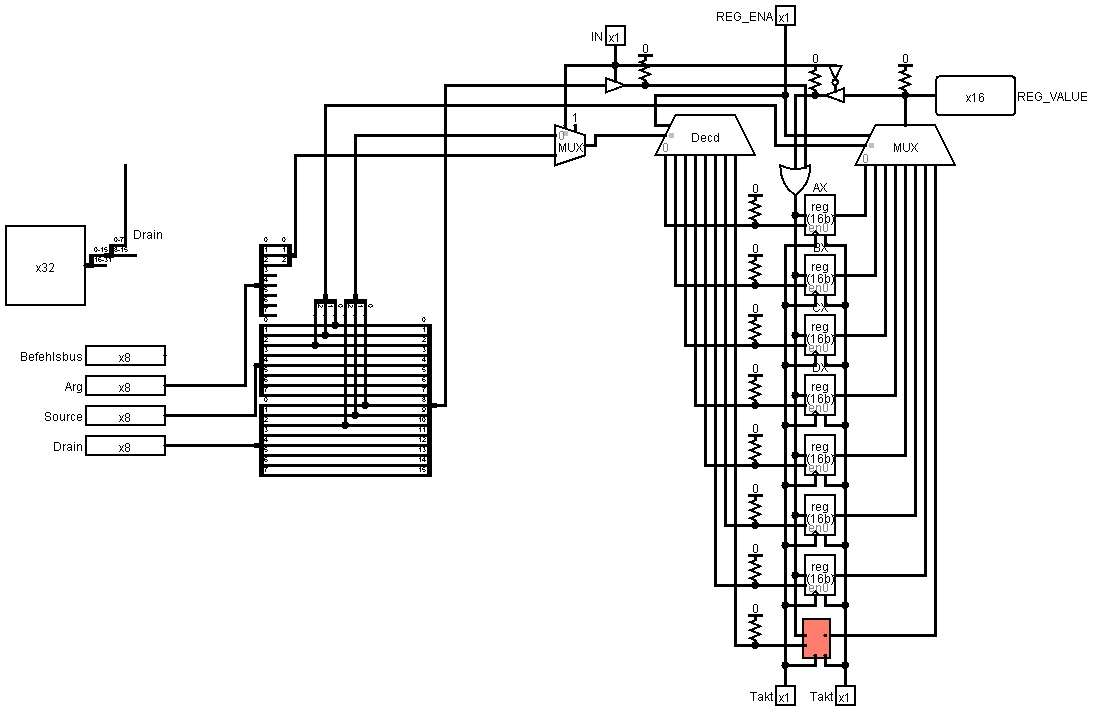
\includegraphics[scale=0.40]{circ}
%\caption{Darstellung des RegisterwerkTODO}
%\centering
%\label{fig:register}
%\end{figure}
\subsection{Adresswerk}

\subsection{Arithmetisch Logische Einheit}
%https://en.wikibooks.org/wiki/Microprocessor_Design/ALU#Example:_4-Bit_ALU
%https://en.wikibooks.org/wiki/Microprocessor_Design
Die ALU (Arithmetic Logic Unit) ist der Teil einer CPU, welcher die eigentliche Datenverarbeitung durchführt. Sie verfügt über keinen eigenen Speicher, die Ergebnisse müssen also in den Registern gespeichert werden. Die ALU ist ein Schaltwerk, welches einfache Operationen auf meist zwei Operanden ausführen kann. So kann das Rechenwerk einer CPU meistens arithmetische, logische und bitschiebende Operationen ausführen. Arithmetische Operationen umfassen Addition und Subtraktion, seltener auch Multiplikation und Division. Addierer und Subtrahierer sind als Hardwareeinheit in die ALU integriert, wohingegen Multiplikation und Division meist algorithmisch durchgeführt werden. Die ALU alleine hat wenig Wirkung, sie obliegt der Kontrolle des Steuerwerkes, das steuert, welche Operation ausgeführt wird, mit welchen Operanden sie ausgeführt wird und in welches Register das Ergebnis gespeichert werden soll.

Rechenwerke sind innerhalb eines Prozessors oft unterschiedlich aufgebaut. 
So haben sehr einfache Prozessoren häufig ein spezielles Register, in welchem das Ergebnis einer ALU Operation automatisch gespeichert wird, den so genannten Akkumulator. Solch ein Register hat den Vorteil, das auf die Angabe eines Zieles bei der Programmierung verzichtet werden kann, da der Ausgang der ALU fest mit dem Akkumulator verbunden ist. Des weiteren ist der Ausgang des Akkumulators fest mit einem der zwei Eingänge der ALU verbunden. Man kann sich den Akkumulator also als fest vorgeschaltetes Register des Rechenwerks vorstellen, in dem auch das Ergebnis gespeichert wird. Deshalb muss bei einer Rechenoperation vom Programmierer nur ein Operand angegeben werden. 

\noindent \textbf{Beispiel:} Wenn im Akkumulator der Wert 10d steht und der Assemblerbefehl ADD RAX ausgeführt wird, dann wird die ALU vom Steuerwerk angewiesen eine Addition auszuführen und übergibt als Parameter am zweiten Eingang den Wert des Registers RAX. Der erste Eingang ist mit dem Akkumulator verbunden und übergibt deshalb den Wert 10d. Das Ergebnis der Berechnung wird wiederum in den Akkumulator gespeichert und überschreibt den vorherigen Wert 10d.  

Diese feste Konfiguration der ALU hat allerdings einige Nachteile weshalb in den meisten modernen Prozessoren eine ALU implementiert ist, die mit keinem Register fest verbunden ist. Eine Rechenwerksoperation muss also immer zwei Quellregister und ein Zielregister angeben. Diese Konfiguration ist zwar sehr flexibel in der Übergabe der Speicherorte, allerdings benötigt sie zusätzliche Schaltungslogik auf dem Chip und die Codekomplexität nimmt zu.


\noindent \textbf{Beispiel:} Bei der Ausführung des Befehls ADD RAX,RBX,RCX werden die Werte der beiden Register RAX und RBX addiert und das Ergebnis in RCX gespeichert.

Die ALU speichert zwar das Ergebnis in dem ihr zugewiesenen Register, allerdings kann der Prozessor keine Eigenschaften der letzten Operation unterscheiden. Diese Fähigkeit wird aber benötigt, wenn der Programmierer beispielsweiße anfordert, dass das Programm an eine andere Adresse springt, sollte das letzte Rechenergebnis 0 ergeben haben. Damit der Prozessor diesen Verlauf der letzten Rechenoperation speichern kann ist den meisten Prozessoren ein Statusregister integriert. Das Statusregister speichert nicht wie die Universalregister einen Wert in mehreren Bits ab, sondern jedes Bit steht im Register für eine bestimmte Eigenschaft der vorhergehenden Rechenoperation. Diese Bits werden Flags genannt. Eine 1 bedeutet dass die letzte Operation diese Bedingung erfüllt hat, eine 0 das Gegenteil. Welche Flags ein Prozessor unterstützt und wie diese angeordnet sind unterscheidet sich von Prozessor zu Prozessor. Allerdings sind die fünf grundlegensten Flags in fast allen Prozessoren implementiert.


\noindent \textbf{Zero-Flag (Nullbit):} Das Zero-Flag ist sehr simpel aufgebaut. Wenn das letzte Ergebnis der ALU gleich Null war wird das Bit auf 1 gesetzt, ansonsten auf 0. Mit diesem Flag lässt sich eine Abbruchbedingung für eine Schleife leicht prüfen. Die Anweisung: $$for(int \ i=5;i \ > \ 0;i--)\{\}$$ wird solange durchlaufen bis das Ergebnis der ALU Operation ($i--$) gleich Null ist und damit das Zero-Flag gesetzt wird. Dann wird die Schleife abgebrochen und der Programmablauf fortgesetzt.

\begin{table}[!htb]
\centering
\caption{Schritte der for-Schleife}
\label{forschleife}
\begin{tabular}{|c|c|c|}
\hline

i & Zero-Flag & Nächster Schritt \\ \hline
5 & 0         & Weiter           \\ \hline
4 & 0         & Weiter           \\ \hline
3 & 0         & Weiter           \\ \hline
2 & 0         & Weiter           \\ \hline
1 & 0         & Weiter           \\ \hline
0 & 1         & Abbruch          \\ \hline
\end{tabular}
\end{table}

Tabelle \ref{forschleife} zeigt die Nutzung des Zero-Flags zur Prüfung der Abbruchbedingung von Abbildung TODO.


\noindent \textbf{Carry-Flag (Übertragsbit):} Das Carry-Flag zeigt an, ob es bei der letzten ALU-Operation zu einem Übertrag gekommen ist. Wie in Abbildung TODO(Übertrag) bereits dargestellt, kommt es zu einem Überlauf, wenn das Ergebnis nicht mehr korrekt mit den vorhandenen Bits dargestellt werden kann. Diese Flag wird beim Rechnen mit vorzeichenlosen Zahlen verwendet.

\begin{table}[!htb]
\centering
\label{carry}
\begin{tabular}{|c|c|c|c|}
\hline
Rechnung & Ergebnis (d) & Ergebnis (b) & Carry-Flag \\ \hline \hline
253+2    & 255          & 11111111     & 0          \\ \hline \hline
253+3    & 256          & 00000000     & 1          \\ \hline
\end{tabular}
\caption{Beispiele Carry-Flag}
\end{table}
In Abbildung \ref{carry} sind beispielhaft zwei Rechenoperationen dargestellt. Es wird angenommen dass die Operation von einer 8-Bit ALU ausgeführt wird. In der ersten Zeile wird die Summe aus 253 und 2 berechnet. Das Ergebnis kann gerade noch als 8-Bit Dualzahl dargestellt werden ($11111111b = 255d$), das Carry-Bit wird deshalb nicht von der ALU gesetzt. Das Ergebnis der Rechnung in der zweiten Zeile  würde neun Bits benötigen um korrekt dargestellt werden zu können ($100000000b = 256d$). Da das Rechenwerk aber nur eine Breite von 8 Bit hat wird im Zielregister der Wert der ersten 8 Bit des Ergebnisses, also null, gespeichert. Um diese Fehlerhafte Rechnung anzuzeigen wird nun das Carry Bit im Flagregister gesetzt.  
Sollte der letzte ausgeführte ALU Befehl ein Schiebebefehl gewesen sein, so wird das Carry Flag dazu verwendet den Wert des herausgeschobenen Bits anzuzeigen.


\noindent \textbf{Sign-Flag (Vorzeichenbit):} Das Vorzeichenbit entspricht dem MSB (most significant bit) des Ergebnisses. Das MSB ist das höchstwertige Bit einer Dualzahl und representiert im Zweierkomplement das Vorzeichen der Zahl.

\noindent \textbf{Overflow-Flag (Überlauf-Bit):} Diese Flag wird beim Rechnen mit Zahlen im Zweierkomplement benötigt. Es wird gesetzt, wenn bei einer Addition oder Subtraktion ein Übertrag auf das MSB stattfindet, also das höchstwertige Bit verändert wird. 
\begin{table}[!htb]
\centering
\label{overflow}
\begin{tabular}{|c|c|c|c|}
\hline
Rechnung (d) & Ergebnis (Zweierkomplement) & Ergebnis (b) & Overflow-Bit \\ \hline \hline
122+5        & 127                         & 01111111     & 0            \\ \hline \hline
122+6        & -128                        & 10000000      & 1            \\ \hline
\end{tabular}
\caption{Rechnen im Zweierkomplement mit 8-Bit Zahlen}
\end{table}

In Abbildung \ref{overflow} sind zwei Rechnungen dargestellt. Im Zweierkomplement hat eine Zahl mit $n$ Bits folgenden darstellbaren Zahlenbereich: 
$${-2}^{n-1}+ ... +2^{n-1}-1$$
In Tabelle \ref{overflow} wird mit 8-Bit Zahlen gearbeitet, also reicht der darstellbare Zahlenbereich für das Beispiel von $-128$ bis $+127$. Die erste Rechnung ergibt 127, die höchste positive darstellbare Zahl im Zweierkomplement mit 8-Bit. Es kommt zu keinem Übertrag auf das MSB, also wird das Overflow Bit nicht gesetzt. In der zweiten Zeile kommt es zu einem Übertrag auf das MSB und das Ergebnis wird verfälscht, da +128 nicht mehr im darstellbaren Zahlenbereich für diese Rechnung liegt. Um das falsche Ergebnis anzuzeigen wird die ALU das Overflow Bit auf 1 setzen. 
%TODO Overflow Flag wird mit XOR aus Carry in und Carry Out berechnet ... Noch nicht ganz verstanden.


\subsection{Memory Management Unit}
%Adressierungsarten

\subsection{Bussysteme}

\section{Speicher}
\subsection{Geschichte}
%https://de.wikipedia.org/wiki/Speicherhierarchie
\subsection{Speicherhierarchie}
\subsection{RAM/ROM}
\subsection{Stack}

\section{Befehlsausführung}
\subsection{Befehlszyklus}
\subsection{Schleifen}
\subsection{Subroutinen}

\section{Besondere Ausführungsarten}
\subsection{Interrupts}
\subsection{Exceptions}


\newpage

\section{Planung und Entwurf eines Prozessors}
Der Inhalt der bisherigen Arbeit handelte von den Komponenten einer CPU und deren Funktionsweißen. Um den dargestellten Inhalt praktischer Vermitteln zu können, wird nun mittels einer Simulationssoftware eine CPU von Grund auf erstellt. Dieser Prozessor stellt keinen Vergleich zu modernen Prozessoren her. Er soll lediglich die Funktionsweiße der essentiellsten Bauteile beschreiben und einfache Operationen wie Sprünge und Subroutinen unterstützen.
\subsection{Befehlsbreite}
Am Anfang der Planung jeder CPU steht die Festlegung der benötigten Befehlsbreite. Je nachdem welche Features eingebaut werden sollen kann der Befehlssatz eingeteilt werden. Logisim bietet die Möglichkeit, einen 32-Bit Bus zu nuzten. Zu Erklärungszwecken werden die 32-Bit wie folgt aufgeteilt:

\begin{table}[!htb]
\centering
\caption{Befehlsbus}
\label{Befehlsbus}
\begin{tabular}{|r|l|}
  \hline
  8-Bit & Opcode \\
  \hline
  8-Bit & Argument \\ 
  \hline
  16-Bit & Value\\
  \hline
  
\end{tabular}
\end{table}

\indent
\textbf{Opcode: } Der Opcode beinhaltet den Befehl welche die CPU als nächstes Ausführen soll(z.B. MOV oder ADD). Es werden nicht mehr als 8-Bit benötigt, da nicht viele Befehle vorhanden sein müssen um die Basisfunktionalität einer CPU zu erzielen.
\newline
\indent
\textbf{Argument: } Das Argument wird nicht bei jedem Befehl verwendet. Diese 8-Bit sind eine Hilfestellung für Operationen bei denen eine genauere Spezifikation der zu ausführenden Tätigkeit benötigt wird. Beispielsweise wird bei der arithmetischen Operation ADD mit Hilfe des Argumentes angegeben, in welches Register das Ergebnis gespeichert werden soll.
\newline
\indent
\textbf{Value: } Die verbleibenden 16-Bit werden als Wertangabe benutzt. Durch diese 16-Bit wird gleichzeitig die Befehlsbusbreite innerhalb des Prozessors festgelegt, das heißt der Prozessor kann mit Zahlen arbeiten welche innerhalb der 16-Bit Grenze liegen (ohne Vorzeichen maximal 65536). Einige Befehle in dieser CPU benötigen allerdings drei Parameter zur Ausführung. Um mit dem Argument drei Parameter bereitzustellen können die letzten 16-Bit in zwei 8-Bit Blöcke gespalten werden. Diese werden hier Quelle und Ziel genannt. Der Befehlssatz sieht bei diesen speziellen Befehlen folgendermaßen aus: 
\begin{table}[!htb]
\centering
\caption{Befehlsbus mit drei Parametern}
\label{Befehlsbus3P}
\begin{tabular}{|r|l|}
  \hline
  8-Bit & Opcode \\
  \hline
  8-Bit & Argument \\ 
  \hline
  8-Bit & Ziel\\
  \hline
  8-Bit & Quelle\\
  \hline
\end{tabular}
\end{table}
\newline
Befehle, welche diese Aufteilung benötigen sind zum Beispiel ALU-Operationen oder der MOV Befehl, welcher den Wert eines Register in ein anderes schiebt.

\subsection{Befehlssatz}

Der Befehlssatz beschreibt die Befehle, welche die CPU ausführen kann.
\newpage
\begin{table}[!htb]
\centering
\caption{Befehlssatz von VI-17}
\begin{tabular}{|r|l|}
  \hline
  00000000 & NOP \\
  \hline
  00000001 & MOV\\ 
  \hline
  00000010 & IN\\
  \hline
  00000011 & STO\\
  \hline
  00000100 & LEA\\
  \hline
  00000101 & PUSH \\ 
  \hline
  00000110 & POP\\
  \hline
  00000111 & -----\\
 \hline
  00001000 & ----- \\
  \hline
  00001001 & CALL\\ 
  \hline
  00001010 & RETURN\\
  \hline
  00001011 & ADD\\
  \hline 
 00001100 & SUB \\
  \hline
  00001101 & INC\\ 
  \hline
  00001110 & DEC\\
  \hline
  00001111 & COMP\\
  \hline
  00010000 & SHIFTL\\
  \hline
  00010001 & SHIFTR\\ 
  \hline
  00010010 & ROTL\\
  \hline
  00010011 & ROTR\\
  \hline
  00010100 & AND\\
  \hline
  00010101 & OR \\ 
  \hline
  00010110 & NOR\\
  \hline
  00010111 & NAND\\
  \hline
  00011000 & XOR\\
  \hline
  00011001 & XNOR \\
  \hline
  00011010 & JIT\\
  \hline
  00011011 & JIF\\
  \hline
  00011100 & JUMP\\
  \hline
\end{tabular}
\end{table}
\newpage
Die CPU soll die grundlegenden Aufgaben eines Prozessors erfüllen können. Die einzelnen Befehle des obigen Befehlssatzes werden nun kurz beschrieben.
\newline
\indent 
\textbf{00000000 NOP: }No Operation. Es wird keine Operation ausgeführt.
\newline
\indent 
\textbf{00000001 MOV: } Move. Überschreibt den Wert des Zielregisters mit dem Wert des Quellregisters. 


\subsection{Speicher}

\subsubsection{RAM/ROM}
\subsubsection{Stack}

\section{Implementierung einer Prozessorsimulation in Logisim}
\subsection{Logisim}
Logisim ist ein Open Source Werkzeug für den Entwurf und die Simulation digitaler Schaltungen. Es bietet die Möglichkeit, größere Schaltungen aus kleineren Schaltungen herzustellen. Damit ist es möglich, ganze Prozessoren in Logisim zu entwerfen. Ein solch einfacher Prozessor soll nun im Folgenden implementiert werden.
\subsection{Prozessor Komponenten}
Der Prozessor besteht aus fünf Hauptkomponenten:
\begin{itemize}
\item Control Unit - Steuerungseinheit
\item ALU - Arithmetisch Logische Einheit
\item Registersatz 
\item RAM/Stack
\item ROM
\end{itemize}

\textbf{Control Unit - Steuerungseinheit: } Die CU verarbeitet die Daten des Befehlsbusses und dekodiert die einzelnen Befehle, welche die CPU als nächstes ausführen muss. Der Befehlsbus wird mittels Komparatoren mit dem gesamtem Befehlssatz verglichen. Wenn ein Befehl gefunden wird sendet die CU die notwendigen Steuersignale an die einzelnen Komponenten des Prozessors, um zum Beispiel die Register zum beschreiben freizuschalten.

\begin{figure}[!htb]
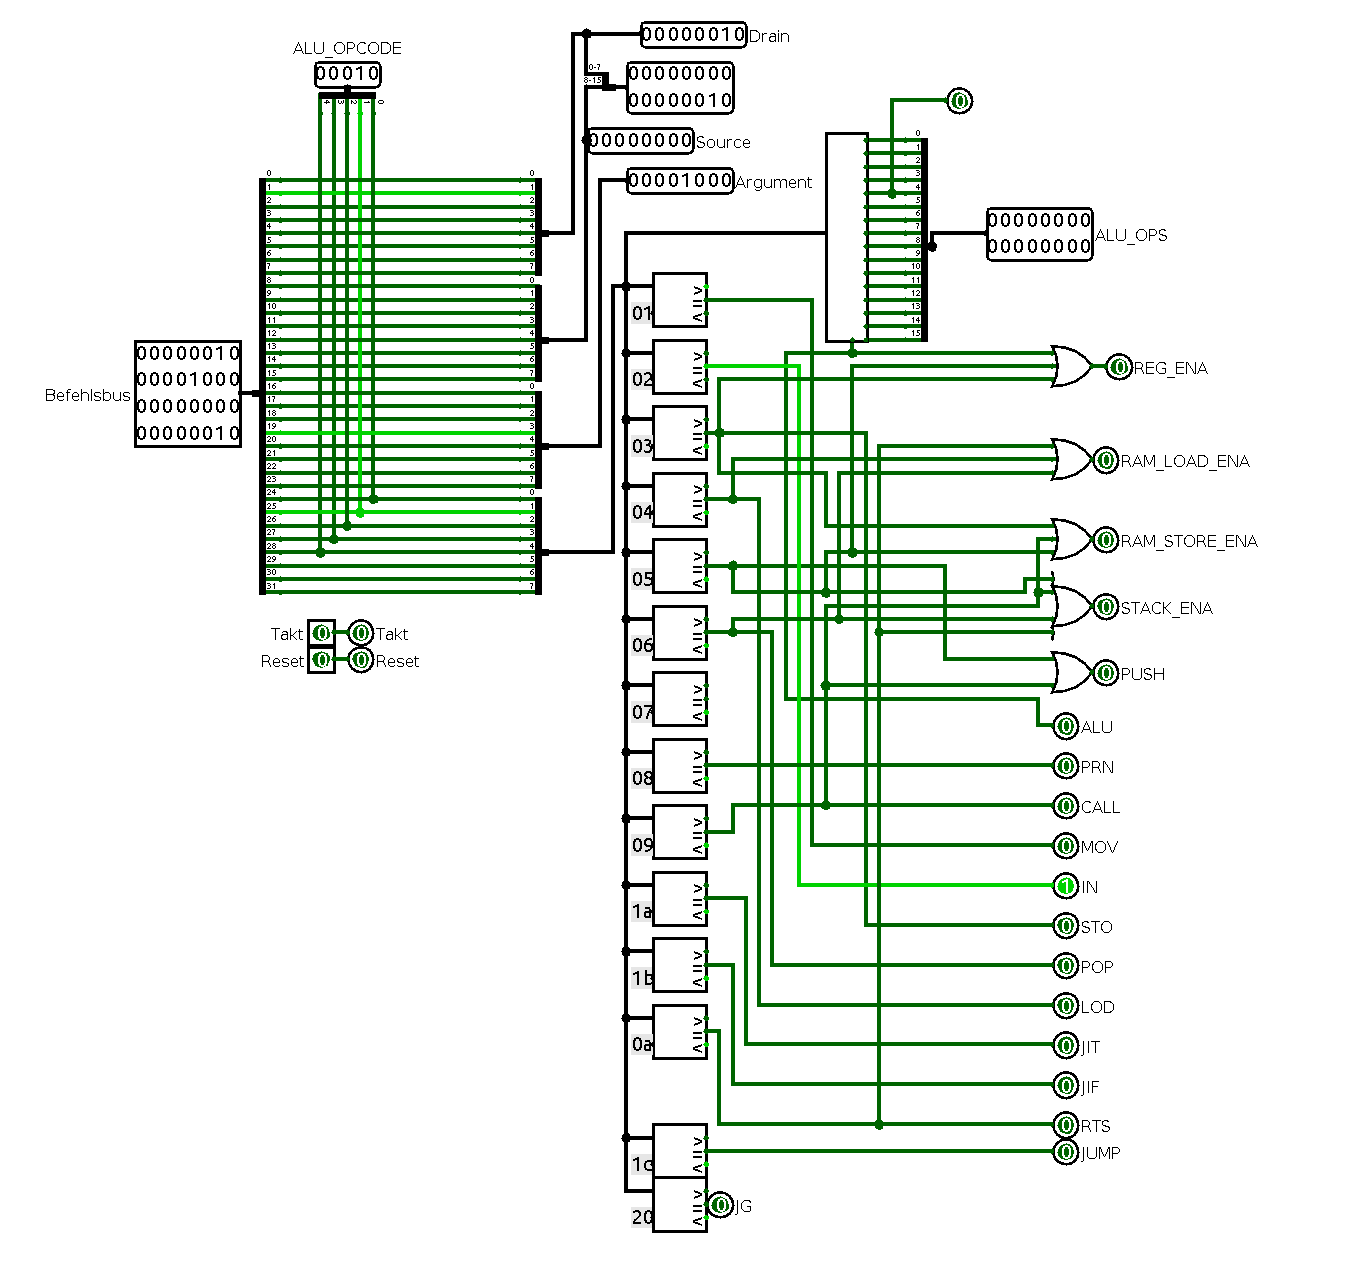
\includegraphics[scale=0.40]{cu}
\caption{Darstellung des Steuerwerks}
\centering
\label{fig:register}
\end{figure}

\newpage
\textbf{Registersatz: }
\begin{figure}[!htb]
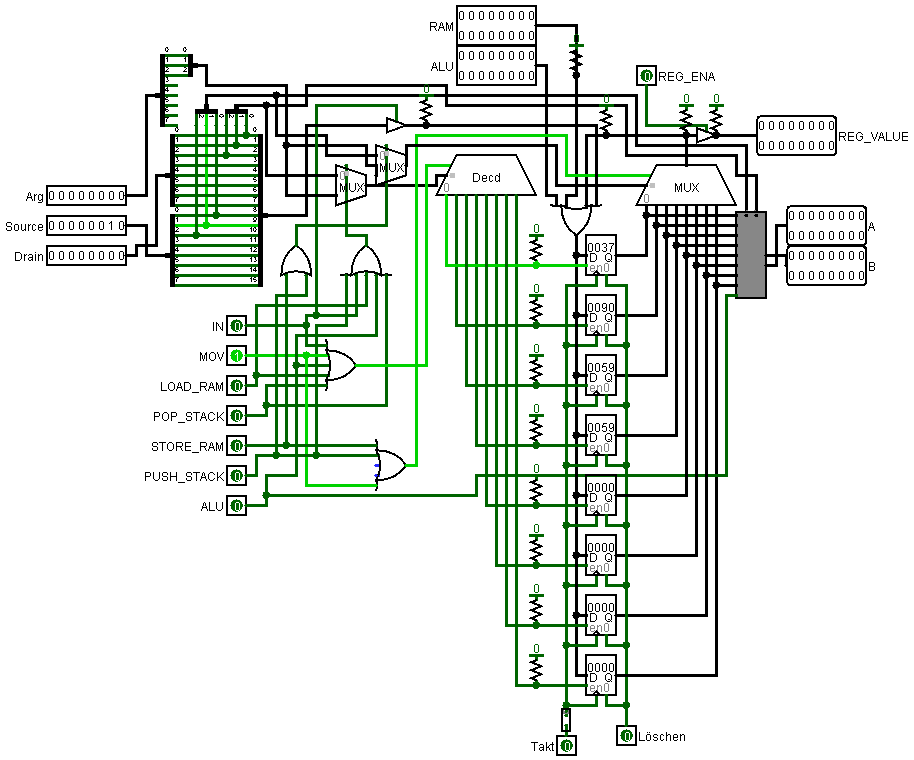
\includegraphics[scale=0.40]{register}
\caption{Darstellung des Registersatzes}
\centering
\label{fig:register}
\end{figure}

\newpage
\subsection{Entwicklung und Ausführung eines Programmes}


Um nun die Funktionalität der CPU zu zeigen wurde ein C++ Programm entwickelt welches alle Primzahlen bis $2^{16} = 65536$ ausrechnet und die Anzahl der Primzahlen auf dem Terminal ausgibt. Dieses Programm wurde unter einem aktuellen Ubuntu kompiliert.

\begin{code}[!htb]
\begin{lstlisting}
bool checkIfPrime(unsigned int x){
	if(x<2) return false;
	unsigned int i=2;
	for(i;i<x;i++){
		if(x%i == 0){
			return false;
		}
	}
	return true;
}

int main(int argc, char const *argv[])
{
	int counter=0;
	for(unsigned int i=1;i<65536;i+=2){
		if(checkIfPrime(i)){
			counter++;
		}s
	}
	std::cout << counter << std::endl; //Ausgabe 6492
	return 0;
}
\end{lstlisting}
\caption[C++ Code Primzahlenzählen]{C++ Code Primzahlenzählen}
\end{code}



Um dieses Programm auf der VI-17 ausführen zu können muss es im Assembler der CPU neu geschrieben werden. Da Assembler eine sehr hardwarenahe Sprache ist, erleichtern wir uns die Entwicklung und betrachten den Assemblercode des C++ Programms, um die grobe Struktur sehen zu können, welche die CPU ausführt. Der Assemblercode kann mittels GDB betrachtet werden. Um den Umfang der Erklärungen nicht zu sprengen muss allerdings ein grundsätzliches Verständnis für den x86 Befehlssatz vorhanden sein.
\newpage


\begin{code}
\begin{lstlisting}
Dump of assembler code for function main:
   0x000000000040085e <+0>:	push   %rbp
   0x000000000040085f <+1>:	mov    %rsp,%rbp
   0x0000000000400862 <+4>:	sub    $0x20,%rsp
   0x0000000000400866 <+8>:	mov    %edi,-0x14(%rbp)
   0x0000000000400869 <+11>:	mov    %rsi,-0x20(%rbp)
   0x000000000040086d <+15>:	movl   $0x0,-0x8(%rbp)
   0x0000000000400874 <+22>:	movl   $0x1,-0x4(%rbp)
   0x000000000040087b <+29>:	cmpl   $0xffff,-0x4(%rbp)
   0x0000000000400882 <+36>:	ja     0x40089c <main+62>
   0x0000000000400884 <+38>:	mov    -0x4(%rbp),%eax
   0x0000000000400887 <+41>:	mov    %eax,%edi
   0x0000000000400889 <+43>:	callq  0x400816 <_Z12checkIfPrimej>
   0x000000000040088e <+48>:	test   %al,%al
   0x0000000000400890 <+50>:	je     0x400896 <main+56>
   0x0000000000400892 <+52>:	addl   $0x1,-0x8(%rbp)
   0x0000000000400896 <+56>:	addl   $0x2,-0x4(%rbp)
   0x000000000040089a <+60>:	jmp    0x40087b <main+29>
   0x000000000040089c <+62>:	mov    -0x8(%rbp),%eax
   0x000000000040089f <+65>:	mov    %eax,%esi
   0x00000000004008a1 <+67>:	mov    $0x601060,%edi
   0x00000000004008a6 <+72>:	callq  0x4006a0 <_ZNSolsEi@plt>
   0x00000000004008ab <+77>:	mov    $0x400700,%esi
   0x00000000004008b0 <+82>:	mov    %rax,%rdi
   0x00000000004008b3 <+85>:	callq  0x4006f0 <_ZNSolsEPFRSoS_E@plt>
   0x00000000004008b8 <+90>:	mov    $0x0,%eax
   0x00000000004008bd <+95>:	leaveq 
   0x00000000004008be <+96>:	retq   
End of assembler dump.
\end{lstlisting}s
\caption[Assemblercode der main Methode]{Assemblercode der main-Methode}
\end{code}

In der Zeile main +15 wird die Variable counter mit 0 initialisiert und auf dem Stack an Offset 0x8 des Base Pointers platziert. 
Anschließend wird die Laufvariable i der for-Schleife in Zeile main+22 mit dem Wert 1 an Offset 0x4 des Base Pointers im Stack initialisiert.
Erster Durchlauf for-Schleife: Zeile +29 Die Laufvariable i wird mit 0xffff (dezimal: 65536) verglichen. Anschließend wird mittels des Assembler-Befehls ja (jump if above) geprüft, welche Flag der vorherige Compare Befehl gesetzt hat. Wenn im Flagregister das greater Bit gesetzt wurde, springt das Programm an die Adresse $0x000000000040089c$ (main+62), also aus for-Schleife raus, da die Schleifenbedingung $(i<65536)$ nicht mehr erfüllt ist. Wenn kein Sprung auftritt, läuft das Programm weiter und ruft an Stelle main+43 die Funktion checkIfPrime auf. Diese Funktion erwartet allerdings einen Übergabeparameter, dieser wird in Register \$edi (main+41)abgelegt. 
Der Rückgabewert der Funktion steht daraufhin, wenn die Funktion durchlaufen und beendet wurde, in Register al. Da checkIfPrime den Rückgabetyp boolean besitzt steht in Register al entweder eine 0 wenn es keine Primzahl war, oder 1 wenn es eine Primzahl war die übergeben wurde. Der Befehl test an Stelle main+48 führt ein bitweise logisches UND zwischen al und al aus. Hier Prüft der Prozessor, ob das Ergebnis ungleich null war und setzt das ZF-Bit (Zero Flag). Wenn das Flag-Bit nicht gesetzt wurde wird das Programm ganz normal weitergeführt. Die counter Variable wird inkrementiert (main+52) und die Laufvariable i wird um zwei erhöht (main+56), daraufhin wird an Stelle main+29 gesprungen und der nächste Schleifendurchgang beginnt.

\begin{code}[!htb]
\begin{lstlisting}
Dump of assembler code for function _Z12checkIfPrimej:
   0x0000000000400816 <+0>:	push   %rbp
   0x0000000000400817 <+1>:	mov    %rsp,%rbp
   0x000000000040081a <+4>:	mov    %edi,-0x14(%rbp)
   0x000000000040081d <+7>:	cmpl   $0x1,-0x14(%rbp)
   0x0000000000400821 <+11>:	ja     0x40082a <_Z12checkIfPrimej+20>
   0x0000000000400823 <+13>:	mov    $0x0,%eax
   0x0000000000400828 <+18>:	jmp    0x40085c <_Z12checkIfPrimej+70>
   0x000000000040082a <+20>:	movl   $0x2,-0x4(%rbp)
   0x0000000000400831 <+27>:	mov    -0x4(%rbp),%eax
   0x0000000000400834 <+30>:	cmp    -0x14(%rbp),%eax
   0x0000000000400837 <+33>:	jae    0x400857 <_Z12checkIfPrimej+65>
   0x0000000000400839 <+35>:	mov    -0x14(%rbp),%eax
   0x000000000040083c <+38>:	mov    $0x0,%edx
   0x0000000000400841 <+43>:	divl   -0x4(%rbp)
   0x0000000000400844 <+46>:	mov    %edx,%eax
   0x0000000000400846 <+48>:	test   %eax,%eax
   0x0000000000400848 <+50>:	jne    0x400851 <_Z12checkIfPrimej+59>
   0x000000000040084a <+52>:	mov    $0x0,%eax
   0x000000000040084f <+57>:	jmp    0x40085c <_Z12checkIfPrimej+70>
   0x0000000000400851 <+59>:	addl   $0x1,-0x4(%rbp)
   0x0000000000400855 <+63>:	jmp    0x400831 <_Z12checkIfPrimej+27>
   0x0000000000400857 <+65>:	mov    $0x1,%eax
   0x000000000040085c <+70>:	pop    %rbp
   0x000000000040085d <+71>:	retq   
End of assembler dump.

\end{lstlisting}
\caption[Assemblercode der checkIfPrime Methode]{Assemblercode der checkIfPrime-Methode}
\end{code}
%Intel Dokumentation zitieren Code Listing 3 URL-
%https://software.intel.com/sites/default/files/managed/a4/60/325383-sdm-vol-2abcd.pdf
Das Code Listing 3 zeigt den Assemblercode der Funktion checkIfPrime. In Zeile 4 wird der Übergabeparameter, welcher sich in Register edi befindet, auf den Stack verschoben. Daraufhin wird mit dem Befehl cmpl dieser Übergabeparameter mit dem Wert 1 verglichen. Dafür werden die beiden Werte subtrahiert und das Ergebnis ausgewertet. Bei dieser Auswertung setzt die CPU automatisch die Flags für die Subtraktion. Wenn Beispielweise eine -2 übergeben wird und vom Befehl compl mit dem Wert 1 verglichen werden soll, so wird die ALU -2-1=-3 rechnen und dabei die Sign Flag(SF) setzen, da das Ergebnis negativ ist. Der nächste Befehl ist jg (Jump if greater), dieser Sprung wird laut Intel-Architektur-Dokumentation nur ausgeführt, wenn die beiden Flags ZF und SF \textbf{nicht} gesetzt, also null, sind. Diese sind null, wenn das Ergebnis zum einen nicht negativ (SF) und nicht null(ZF) ist. \newline Kurz gesagt: Die beiden Zeilen 7 und 11 stellen sicher, dass der Übergabeparameter größer als 1 ist. Im C++ Programm entspricht das der ersten Zeile der Funktion. Sollte eine der beiden Flags ZF bzw. SF nicht gesetzt sein, wird nicht gesprungen und in Zeile 13 eine 0 in das Rückgaberegister geschrieben. Daraufhin wird zum Ende der Funktion gesprungen und die Funktion ist beendet. Wenn der Sprung in Zeile 11 ausgeführt wird, dann springt das Programm zu Zeile 20 in der die Laufvariable i  mit dem Wert 2 initialisiert wird. Die Zeilen 27 bis 30 sind analog zu Codelisting 2 die Prüfung der Laufvariable in der for-Schleife, ob die Abbruchbedinggung bereits erfüllt ist. In der Schleife werden die Zeilen 35 bis 59 ausgeführt. Der Befehl idvl führt eine Division aus, wobei der Rest in Register EDX gespeichert wird. Nachdem EDX in EAX verschoben wurde wird mittels des Befehls test EAX,EAX (Zeile 48) geprüft, ob das Register null ist, also auch der Rest der Division null ist. Sollte dem so sein, so springt das Programm ans Ende und schreibt eine 0 in Übergaberegister EAX.


\newpage
\bibliography{Referenzen}

\end{document}



















